\documentclass{article}

\usepackage[a4paper, total={6.5in, 11in}]{geometry}
\usepackage{graphicx}
\graphicspath{{titech/CSC.T463.ComputerGraphics/h2/}}

\usepackage{latex/common}

\title{Computer Graphics 2021 - Assignment 2}
\author{Sixue Wang\\21M30927\\Tokyo Institute of Technology}

\begin{document}

\maketitle

\section{Graph}
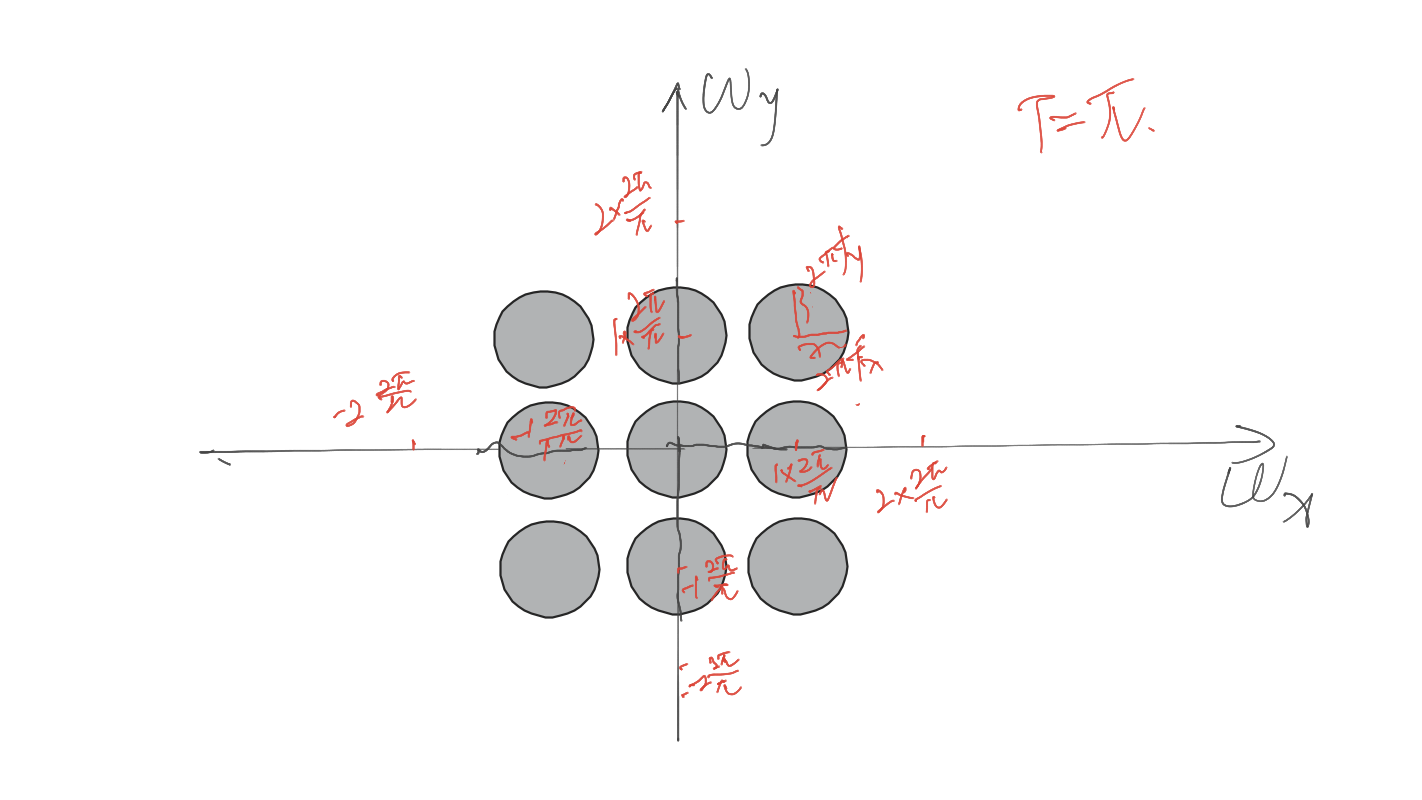
\includegraphics[width=\textwidth]{h2_1.png}

\section{}
In the above figure, every center of the ellipse is at $(N_x*\frac{2\pi}{\pi}, N_y*\frac{2\pi}{\pi}), N_x,N_y=-\infty,...,\infty$. The x-radius is $2\pi$ times $f_x$ the frequency of x in the signal domain and the y-radius is $2\pi$ times $f_y$ the frequency of y in the signal domain. We say aliasing if two ellipses overlap. Then aliasing-free means $2*2\pi f_x < \frac{2\pi}{\pi}$ and $2*2\pi f_y < \frac{2\pi}{\pi}$. So the highest frequency of x and y are both $\frac{1}{2\pi}$.


\end{document}
